\documentclass{article}
\usepackage[utf8]{inputenc}

\usepackage{tikz}
\usetikzlibrary{positioning, fit}

\begin{document}

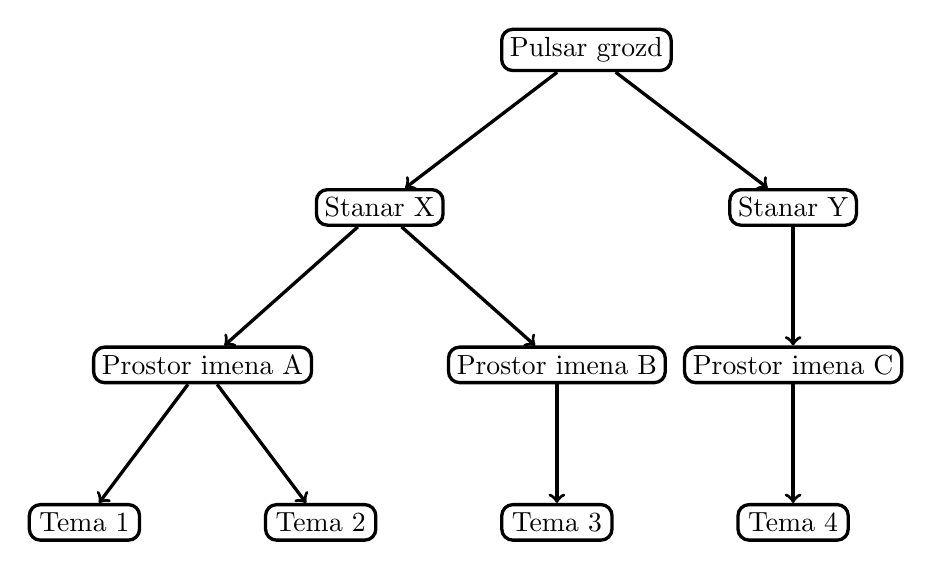
\begin{tikzpicture}[ % has a lot of options; consult the pgf manual
bend angle=15,
long_square/.style={rectangle, draw=black, fill=white, very thick, inner sep=3pt, minimum width=14mm},
rounded_square/.style={rectangle, rounded corners, draw=black, fill=white, very thick, inner sep=3pt, minimum width=14mm},
empty_circle/.style={rectangle, rounded corners=2mm, draw=black, fill=white, very thick, minimum size=4mm},
point/.style={circle, inner sep=0mm},
fit_square/.style={rectangle, rounded corners=2mm, draw=black, very thick, minimum height=20mm,  minimum width=50mm},
both_arrow/.style={<->, very thick},
out_arrow/.style={->, very thick},
in_arrow/.style={<-, very thick},
above_edge_text/.style={above, midway, sloped}
]

\node[rounded_square](cluster) at (6.375,0) {Pulsar grozd};

\node[rounded_square](tenant_1) at (3.75,-2) {Stanar X};
\node[rounded_square](tenant_2) at (9,-2) {Stanar Y};

\node[rounded_square](namespace_1) at (1.5,-4) {Prostor imena A};
\node[rounded_square](namespace_2) at (6,-4) {Prostor imena B};
\node[rounded_square](namespace_3) at (9,-4) {Prostor imena C};

\node[rounded_square](topic_1) at (0,-6) {Tema 1};
\node[rounded_square](topic_2) at (3,-6) {Tema 2};
\node[rounded_square](topic_3) at (6,-6) {Tema 3};
\node[rounded_square](topic_4) at (9,-6) {Tema 4};



\draw[out_arrow](cluster) to [] node[auto]{} (tenant_1);
\draw[out_arrow](cluster) to [] node[auto]{} (tenant_2);

\draw[out_arrow](tenant_1) to [] node[auto]{} (namespace_1);
\draw[out_arrow](tenant_1) to [] node[auto]{} (namespace_2);
\draw[out_arrow](tenant_2) to [] node[auto]{} (namespace_3);

\draw[out_arrow](namespace_1) to [] node[auto]{} (topic_1);
\draw[out_arrow](namespace_1) to [] node[auto]{} (topic_2);
\draw[out_arrow](namespace_2) to [] node[auto]{} (topic_3);
\draw[out_arrow](namespace_3) to [] node[auto]{} (topic_4);

\end{tikzpicture}

\end{document}